%% ============================================================
%%  Memory Controller -- DDR Memories  |  Beamer Presentation
%%  Compile with:  pdflatex DFI_PHY_v4.tex  (run twice)
%% ============================================================
\documentclass[aspectratio=169,10pt]{beamer}

\usetheme{Madrid}
\usecolortheme{default}

\definecolor{ddrblue}{RGB}{10,60,100}
\definecolor{ddrteal}{RGB}{0,130,140}
\definecolor{ddraccent}{RGB}{0,190,180}
\definecolor{ddrgold}{RGB}{230,170,0}
\definecolor{ddrlight}{RGB}{235,245,250}
\definecolor{ddrred}{RGB}{180,30,30}
\definecolor{ddrgreen}{RGB}{20,130,80}
\definecolor{ddrgray}{RGB}{90,100,110}

\setbeamercolor{palette primary}{bg=ddrblue,fg=white}
\setbeamercolor{palette secondary}{bg=ddrteal,fg=white}
\setbeamercolor{palette tertiary}{bg=ddrblue,fg=white}
\setbeamercolor{palette quaternary}{bg=ddrblue,fg=white}
\setbeamercolor{structure}{fg=ddrblue}
\setbeamercolor{block title}{bg=ddrblue,fg=white}
\setbeamercolor{block body}{bg=ddrlight,fg=black}
\setbeamercolor{frametitle}{bg=ddrblue,fg=white}
\setbeamercolor{title}{bg=ddrblue,fg=white}
\setbeamercolor{author}{fg=white}
\setbeamercolor{institute}{fg=white}

\setbeamerfont{frametitle}{size=\large,series=\bfseries}
\setbeamerfont{title}{size=\Large,series=\bfseries}

\usepackage{tikz}
\usetikzlibrary{arrows.meta,positioning,shapes.geometric,
                fit,backgrounds,decorations.markings,
                patterns,calc,matrix,chains,decorations.pathreplacing}
\usepackage{pgfplots}
\pgfplotsset{compat=1.18}
\usepackage{booktabs}
\usepackage{colortbl}
\usepackage{xcolor}
\usepackage{amsmath}
\usepackage{siunitx}
\usepackage{microtype}

\tikzset{
  box/.style={rectangle,rounded corners=3pt,draw=#1!70,fill=#1!12,
              text=black,minimum height=7mm,minimum width=22mm,
              font=\footnotesize\bfseries,align=center},
  box/.default=ddrblue,
  arr/.style={-{Stealth[length=5pt]},thick,#1},
  arr/.default=ddrblue,
  phy/.style={rectangle,rounded corners=4pt,draw=ddrteal,
              fill=ddrteal!15,minimum height=8mm,minimum width=24mm,
              font=\footnotesize\bfseries,align=center},
  ddrbox/.style={rectangle,rounded corners=3pt,draw=#1,fill=#1!15,
                 minimum height=7mm,minimum width=20mm,
                 font=\scriptsize\bfseries,align=center},
}

%% Footline: slide number only (right side), no author/title
\setbeamertemplate{navigation symbols}{}
\setbeamertemplate{headline}{%
  \begin{beamercolorbox}[wd=\paperwidth,ht=12.5ex,dp=1.5ex]{}
    \vspace{4pt}\hfill
    
\includegraphics[height=0.85cm]{images/chips_logo.png}%
    \hspace{0.3cm}
  \end{beamercolorbox}%
}
\setbeamertemplate{footline}{%
  \leavevmode
  \hbox{%
    \begin{beamercolorbox}[wd=\paperwidth,ht=2.25ex,dp=1ex,right]{palette tertiary}%
      \usebeamerfont{date in head/foot}%
      \insertframenumber{} / \inserttotalframenumber\hspace{6pt}
    \end{beamercolorbox}}%
  \vskip0pt%
}

\title{Memory Controllers for DDR Memories}
\subtitle{Signal Integrity, Lane Skew \& PHY Interface}
\author{%
  Pranav M \texttt{PES2UG23EC076}\\[4pt]
  Lalith \texttt{PES2UG23EC074}\\[4pt]
  Harshini S \texttt{PES2UG23EC058}%
}
\institute{Centre for Heterogeneous \& Intelligent Processing Systems\\PES University}
\date{}

% ════════════════════════════════════════════════════════════
\begin{document}
% ════════════════════════════════════════════════════════════

%% ── SLIDE 0 – Title ─────────────────────────────────────────
\begin{frame}
  \begin{beamercolorbox}[wd=\paperwidth,ht=0.22\paperheight,dp=0pt,
      center,sep=10pt]{frametitle}
    \usebeamerfont{title}\color{white}\inserttitle
  \end{beamercolorbox}
  \vspace{28pt}
  \begin{center}
    \begin{tabular}{rl}
      \textbf{Pranav M}   & \texttt{PES2UG23EC076}\\[8pt]
      \textbf{Lalith}     & \texttt{PES2UG23EC074}\\[8pt]
      \textbf{Harshini S} & \texttt{PES2UG23EC058}\\
    \end{tabular}
  \end{center}
\end{frame}

%% ── SLIDE 1 – Recap ─────────────────────────────────────────
\begin{frame}{Recap: Memory Controller for DDR Memories}
\begin{columns}[T]

\begin{column}{0.36\textwidth}
  \vspace{6pt}
  \begin{itemize}\setlength\itemsep{8pt}
    \item Acts as a bridge between the SoC and DRAM
    \item Enforces 50+ timing constraints (tWTR, tRC, tFAW\ldots)
    \item Handles row-buffer management and request scheduling
    \item Manages power modes: PASR, TCSR, Deep Power-Down
    \item AXI out-of-order IDs map naturally to DDR bank parallelism
  \end{itemize}
\end{column}

\begin{column}{0.62\textwidth}
  \centering
  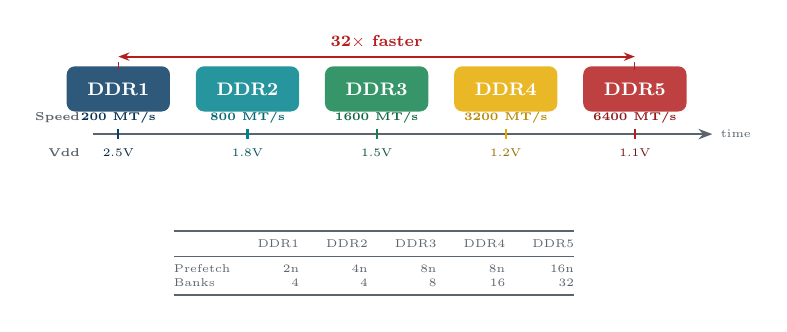
\begin{tikzpicture}[scale=0.82, transform shape]
    %% Timeline axis
    \draw[-{Stealth[length=5pt]},thick,ddrgray] (-0.4,0) -- (9.2,0)
          node[right,font=\tiny,ddrgray]{time};

    \foreach \gen/\speed/\vdd/\col/\x in {
      DDR1/{200 MT/s}/{2.5V}/ddrblue/0,
      DDR2/{800 MT/s}/{1.8V}/ddrteal/2.0,
      DDR3/{1600 MT/s}/{1.5V}/ddrgreen/4.0,
      DDR4/{3200 MT/s}/{1.2V}/ddrgold/6.0,
      DDR5/{6400 MT/s}/{1.1V}/ddrred/8.0}{
      \node[rectangle,rounded corners=3pt,fill=\col!85,text=white,
            font=\footnotesize\bfseries,minimum width=16mm,minimum height=7mm,
            align=center] at (\x,0.70) {\gen};
      \draw[\col,thick] (\x,0.08)--(\x,-0.08);
      \node[font=\fontsize{5pt}{6pt}\selectfont\bfseries,text=\col!80!black]
            at (\x, 0.26) {\speed};
      \node[font=\fontsize{5pt}{6pt}\selectfont,text=\col!65!black]
            at (\x,-0.28) {\vdd};
    }
    \node[font=\fontsize{5pt}{6pt}\selectfont\bfseries,ddrgray,left=2pt]
          at (-0.4, 0.26) {Speed};
    \node[font=\fontsize{5pt}{6pt}\selectfont\bfseries,ddrgray,left=2pt]
          at (-0.4,-0.28) {Vdd};

    %% 32x annotation
    \draw[ddrred,thick,{Stealth[length=4pt]}-{Stealth[length=4pt]}]
      (0,1.20) -- node[above,font=\scriptsize\bfseries,ddrred]{32$\times$ faster} (8.0,1.20);
    \draw[ddrred,dashed,thin] (0,1.12)--(0,0.98);
    \draw[ddrred,dashed,thin] (8.0,1.12)--(8.0,0.98);

    %% Feature table — moved lower to avoid overlap
    \node[font=\fontsize{5pt}{6pt}\selectfont,align=center,ddrgray] at (4.0,-2.0) {%
      \begin{tabular}{@{}lrrrrr@{}}
        \toprule
                 & DDR1 & DDR2 & DDR3 & DDR4 & DDR5\\
        \midrule
        Prefetch & 2n & 4n & 8n & 8n  & 16n\\
        Banks    & 4  & 4  & 8  & 16  & 32 \\
        \bottomrule
      \end{tabular}
    };
  \end{tikzpicture}
\end{column}

\end{columns}
\end{frame}

%% ── SLIDE 2 – System Block Diagram ──────────────────────────
\begin{frame}{System Block Diagram}
\centering
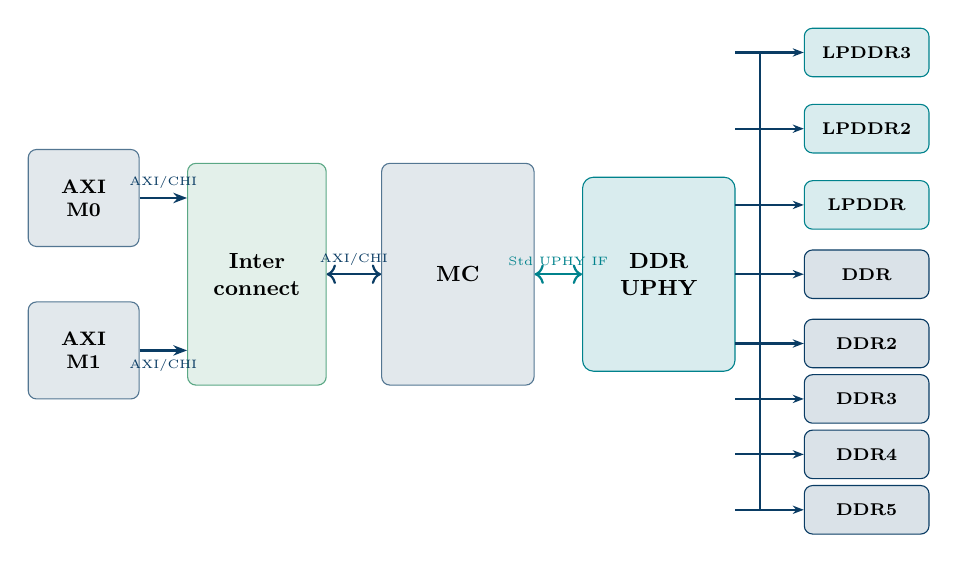
\begin{tikzpicture}[scale=0.88, transform shape]

  \node[box=ddrblue,minimum width=16mm,minimum height=14mm] (m0) at (0,1.1)  {AXI\\M0};
  \node[box=ddrblue,minimum width=16mm,minimum height=14mm] (m1) at (0,-1.1) {AXI\\M1};

  \node[box=ddrgreen,minimum width=20mm,minimum height=32mm,font=\small\bfseries]
        (ic) at (2.5,0) {Inter\\connect};

  \node[box=ddrblue,minimum width=22mm,minimum height=32mm,font=\small\bfseries]
        (mc) at (5.4,0) {MC};

  \node[phy,minimum width=22mm,minimum height=28mm,font=\small\bfseries]
        (phy) at (8.3,0) {DDR\\UPHY};

  \foreach \name/\y/\col in {
    LPDDR3/3.2/ddrteal, LPDDR2/2.1/ddrteal, LPDDR/1.0/ddrteal,
    DDR/0.0/ddrblue, DDR2/-1.0/ddrblue, DDR3/-1.8/ddrblue,
    DDR4/-2.6/ddrblue, DDR5/-3.4/ddrblue}{
    \node[ddrbox=\col,minimum width=18mm] (\name) at (11.3,\y) {\name};
  }

  \draw[arr] (m0.east) -- node[above,font=\tiny]{AXI/CHI} (m0.east -| ic.west);
  \draw[arr] (m1.east) -- node[below,font=\tiny]{AXI/CHI} (m1.east -| ic.west);
  \draw[arr=ddrblue,<->] (ic.east) -- node[above,font=\tiny]{AXI/CHI} (mc.west);
  \draw[arr=ddrteal,<->] (mc.east) -- node[above,font=\tiny]{Std UPHY IF} (phy.west);

  \foreach \name in {LPDDR3,LPDDR2,LPDDR,DDR,DDR2,DDR3,DDR4,DDR5}{
    \draw[arr=ddrblue,-{Stealth[length=4pt]}]
      (phy.east |- \name.west) -- (\name.west);
  }
  \draw[thick,ddrblue] (phy.east) -- ++(0.35,0) |-($(LPDDR3.west)+(-0.35,0)$);
  \draw[thick,ddrblue] ($(phy.east)+(0.35,0)$)  |-($(DDR5.west)+(-0.35,0)$);

\end{tikzpicture}
\end{frame}

%% ── SLIDE 3 – Inter-Lane Skew ───────────────────────────────
\begin{frame}{Inter-Lane Skew: Off-Die Signal Integrity}
\begin{columns}[T]

\begin{column}{0.40\textwidth}
  \vspace{6pt}
  \begin{itemize}\setlength\itemsep{8pt}
    \item DDR transfers data in parallel across multiple DQ byte lanes
    \item Each lane follows a different PCB path, picking up delay $\delta_i$
    \item Skew window: $W_\delta = \max(\delta_i) - \min(\delta_i)$
    \item DDR5 UI $\approx$ 156\,ps; 20\,ps skew eats $>$12\% of it
    \item PHY training (Write Levelling, DQS Gating) corrects $\delta_i$ per lane
  \end{itemize}
\end{column}

\begin{column}{0.56\textwidth}
  \vspace{14pt}
  \centering
  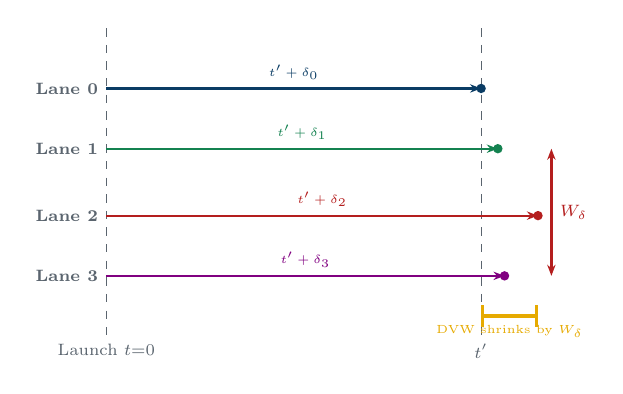
\begin{tikzpicture}[scale=0.85, transform shape]
    \draw[dashed,ddrgray,thin] (0,0.3) -- (0,-4.3)
          node[below,font=\scriptsize]{Launch $t{=}0$};
    \draw[dashed,ddrgray,thin] (5.6,0.3) -- (5.6,-4.3)
          node[below,font=\scriptsize]{$t'$};

    \colorlet{lc0}{ddrblue}
    \colorlet{lc1}{ddrgreen}
    \colorlet{lc2}{ddrred}
    \colorlet{lc3}{violet}

    \foreach \i/\y/\lc/\dx in {0/-0.6/lc0/0, 1/-1.5/lc1/0.25,
                                2/-2.5/lc2/0.85, 3/-3.4/lc3/0.35}{
      \node[left,font=\scriptsize\bfseries,ddrgray] at (0,\y) {Lane \i};
      \draw[\lc,thick,-{Stealth[length=4pt]}] (0,\y)
        -- node[midway,above,font=\tiny,\lc]{$t'+\delta_\i$}
           (5.6+\dx,\y);
      \fill[\lc] (5.6+\dx,\y) circle (2pt);
    }

    \draw[thick,ddrred,{Stealth[length=4pt]}-{Stealth[length=4pt]}]
          (6.65,-1.5) -- node[right,font=\scriptsize,ddrred]{$W_\delta$}
          (6.65,-3.4);

    \draw[ddrgold,very thick,|-|] (5.60,-4.0) --
      node[below,font=\tiny,ddrgold]{DVW shrinks by $W_\delta$} (6.45,-4.0);
  \end{tikzpicture}
\end{column}

\end{columns}
\end{frame}

%% ── SLIDE 4 – Off-Die vs On-Die Delay ──────────────────────
\begin{frame}{Off-Die vs On-Die Delay}
\begin{columns}[T]

\begin{column}{0.3\textwidth}
  \vspace{2pt}
  {\small\textbf{\color{ddrblue}Off-Die (Picoseconds)}}
  \begin{itemize}\setlength\itemsep{2pt}\small
    \item Signals traverse PCB traces, vias
    \item FR4 velocity $\approx 0.6c$; $\sim$1\,ps per 180\,\si{\micro m}
    \item 30\,mm trace $\approx$ 170\,ps; $W_\delta$ typically 5--50\,ps
  \end{itemize}
  \vspace{5pt}
  {\small\textbf{\color{ddrteal}On-Die (Femto/Attoseconds)}}
  \begin{itemize}\setlength\itemsep{2pt}\small
    \item nm-scale on-chip metal interconnect
    \item 1\,\si{\micro m} wire $\approx$ 3--10\,as propagation
    \item Gate delay (3\,nm): 1--5\,ps; bottleneck is logic depth
  \end{itemize}
  \vspace{5pt}
  {\small\textit{PCB/package is the timing bottleneck, not the silicon.}}
\end{column}

\begin{column}{0.58\textwidth}
  \vspace{8pt}
  \centering
  %% PCB trace diagram
  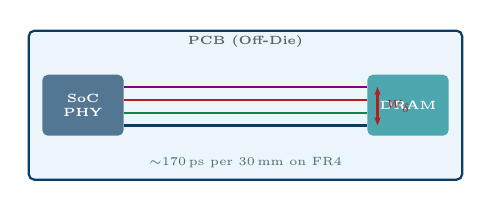
\begin{tikzpicture}[scale=0.86, transform shape]
    \fill[ddrlight,rounded corners=4pt] (0,0) rectangle (6.4,2.2);
    \draw[ddrblue,thick,rounded corners=2pt] (0,0) rectangle (6.4,2.2);
    \node[font=\tiny\bfseries,ddrgray] at (3.2,2.04) {PCB (Off-Die)};

    \fill[ddrblue!70,rounded corners=2pt] (0.2,0.65) rectangle (1.4,1.55);
    \node[white,font=\tiny\bfseries,align=center] at (0.80,1.10) {SoC\\PHY};

    \fill[ddrteal!70,rounded corners=2pt] (5.0,0.65) rectangle (6.2,1.55);
    \node[white,font=\tiny\bfseries] at (5.60,1.10) {DRAM};

    \foreach \y/\col in {0.80/ddrblue, 0.99/ddrgreen, 1.18/ddrred, 1.37/violet}{
      \draw[\col,thick] (1.4,\y) -- (5.0,\y);
    }
    \draw[{Stealth[length=3pt]}-{Stealth[length=3pt]},ddrred,thick]
         (5.15,0.80) -- node[right,font=\tiny,ddrred]{$W_\delta$} (5.15,1.37);
    \node[font=\tiny,ddrgray] at (3.2,0.25) {$\sim$170\,ps per 30\,mm on FR4};
  \end{tikzpicture}

  \vspace{10pt}

  %% Time-scale bar diagram
  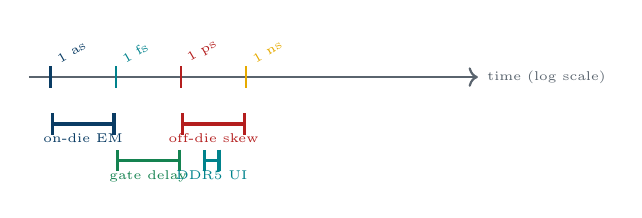
\begin{tikzpicture}[scale=0.92, transform shape]
    \draw[thick,ddrgray,->] (0,0) -- (6.2,0)
          node[right,font=\tiny]{time (log scale)};
    \foreach \x/\lab/\col in {
      0.3/{1 as}/ddrblue, 1.2/{1 fs}/ddrteal,
      2.1/{1 ps}/ddrred,  3.0/{1 ns}/ddrgold}{
      \draw[\col,thick] (\x,-0.15)--(\x,0.15);
      \node[\col,font=\tiny,rotate=30,anchor=west] at (\x,0.18) {\lab};
    }
    \draw[ddrblue,very thick,|-|] (0.3,-0.65)
          -- node[below,font=\tiny,ddrblue]{on-die EM} (1.2,-0.65);
    \draw[ddrgreen,very thick,|-|] (1.2,-1.15)
          -- node[below,font=\tiny,ddrgreen]{gate delay} (2.1,-1.15);
    \draw[ddrred,very thick,|-|] (2.1,-0.65)
          -- node[below,font=\tiny,ddrred]{off-die skew} (3.0,-0.65);
    \draw[ddrteal,very thick,|-|] (2.4,-1.15)
          -- node[below,font=\tiny,ddrteal]{DDR5 UI} (2.65,-1.15);
  \end{tikzpicture}
\end{column}

\end{columns}
\end{frame}

%% ── SLIDE 5 – Why Picoseconds Matter ───────────────────────
\begin{frame}{Why Picoseconds Matter at Modern DDR Speeds}
\begin{columns}[T]

\begin{column}{0.52\textwidth}
  \centering
  \vspace{4pt}
  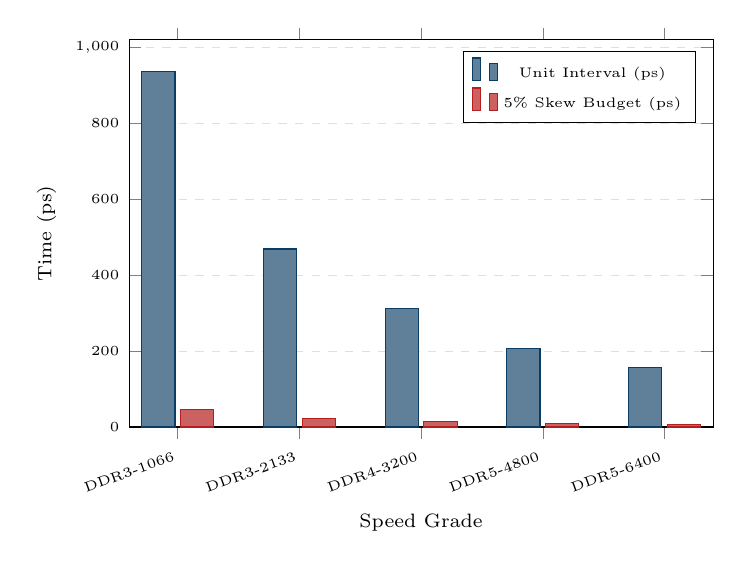
\begin{tikzpicture}
    \begin{axis}[
      ybar, bar width=12pt,
      width=9.0cm, height=6.5cm,
      xlabel={Speed Grade},
      ylabel={Time (ps)},
      xtick={1,2,3,4,5},
      xticklabels={DDR3-1066, DDR3-2133, DDR4-3200, DDR5-4800, DDR5-6400},
      xticklabel style={font=\tiny, rotate=20, anchor=north east},
      yticklabel style={font=\tiny},
      xlabel style={font=\scriptsize},
      ylabel style={font=\scriptsize},
      ymajorgrids=true,
      grid style={dashed,gray!25},
      legend style={font=\tiny, at={(0.97,0.97)}, anchor=north east},
      ymin=0, ymax=1020,
    ]
      \addplot[fill=ddrblue!65, draw=ddrblue] coordinates
        {(1,937)(2,469)(3,312)(4,208)(5,156)};
      \addplot[fill=ddrred!70, draw=ddrred] coordinates
        {(1,46.9)(2,23.4)(3,15.6)(4,10.4)(5,7.8)};
      \legend{Unit Interval (ps), 5\% Skew Budget (ps)}
    \end{axis}
  \end{tikzpicture}
\end{column}

\begin{column}{0.44\textwidth}
  \vspace{6pt}
  \centering
  \rowcolors{2}{ddrlight}{white}
  \begin{tabular}{@{}lrr@{}}
    \toprule
    \textbf{Speed} & \textbf{UI} & \textbf{5\% Budget}\\
    \midrule
    DDR3-1066 & 937\,ps & 46.9\,ps\\
    DDR3-2133 & 469\,ps & 23.4\,ps\\
    DDR4-3200 & 312\,ps & 15.6\,ps\\
    DDR5-4800 & 208\,ps & 10.4\,ps\\
    DDR5-6400 & 156\,ps & \textcolor{ddrred}{\textbf{7.8\,ps}}\\
    \bottomrule
  \end{tabular}

  \vspace{6pt}
  \begin{itemize}\setlength\itemsep{4pt}\small
    \item At DDR5-6400 the skew budget is just \textbf{7.8\,ps}
    \item Uncompensated off-die skew can fill this entirely
    \item PHY training trims $\delta_i$ to $\ll$5\,ps per lane
  \end{itemize}
\end{column}

\end{columns}
\end{frame}

%% ── SLIDE 6 – DFI Interface ─────────────────────────────────
\begin{frame}{DFI: The Standard MC--PHY Interface}
\begin{columns}[T]

\begin{column}{0.38\textwidth}
  \vspace{6pt}
  \begin{itemize}\setlength\itemsep{8pt}
    \item \textbf{DFI} is the industry-standard interface between MC and DDR PHY
    \item Decouples MC from PHY implementation details
    \item Covers command, data, training and power signals
    \item DFI 5.1: PHY-independent boot, expanded freq range, enhanced calibration feedback
  \end{itemize}
\end{column}

\begin{column}{0.58\textwidth}
  \centering
  \vspace{4pt}
  %% MC -- PHY -- DRAM chain
  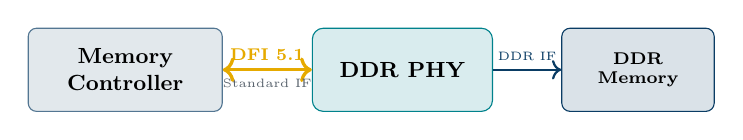
\begin{tikzpicture}[scale=0.88, transform shape]
    \node[box=ddrblue,minimum width=28mm,minimum height=12mm,font=\small\bfseries]
      (mc) at (0,0) {Memory\\Controller};
    \node[phy,minimum width=26mm,minimum height=12mm,font=\small\bfseries]
      (phy) at (4.0,0) {DDR PHY};
    \node[ddrbox=ddrblue,minimum width=22mm,minimum height=12mm]
      (ddr) at (7.4,0) {DDR\\Memory};
    \draw[arr=ddrgold,<->,very thick]
      (mc.east) -- node[above,font=\scriptsize\bfseries,ddrgold]{DFI 5.1}
                   node[below,font=\tiny,ddrgray]{Standard IF} (phy.west);
    \draw[arr=ddrblue,->]
      (phy.east) -- node[above,font=\tiny]{DDR IF} (ddr.west);
  \end{tikzpicture}

  \vspace{10pt}

  %% Version table
  \rowcolors{2}{ddrlight}{white}
  {\scriptsize
  \begin{tabular}{@{}clp{22mm}@{}}
    \toprule
    \textbf{Ver} & \textbf{Key Addition} & \textbf{Support}\\
    \midrule
    1.0 & Initial spec          & DDR, DDR2\\
    2.0 & Training interface    & DDR3, LPDDR2\\
    3.0 & Low-power handshake   & DDR4, LPDDR4\\
    4.0 & DDR5 read/write paths & DDR5\\
    5.0 & PHY-independent boot  & DDR5, LPDDR5\\
    \rowcolor{ddrgold!30}
    \textbf{5.1} & \textbf{Full back-compat} & \textbf{All gens}\\
    \bottomrule
  \end{tabular}}
\end{column}

\end{columns}
\end{frame}

%% ── SLIDE 7 – DFI 5.1 Key Features ─────────────────────────
\begin{frame}{DFI 5.1 Key Features}
\begin{columns}[T]

\begin{column}{0.48\textwidth}
  \vspace{6pt}
  \textbf{\color{ddrblue}Three pillars of DFI 5.1}
  \begin{enumerate}\setlength\itemsep{8pt}
    \item \textbf{PHY-Independent Boot}\\
          MC initialises DRAM without knowing PHY internals
    \item \textbf{Expanded Frequency Range}\\
          Covers low-power LPDDR through DDR5-6400
    \item \textbf{Enhanced PHY$\leftrightarrow$MC Interaction}\\
          Real-time calibration feedback and margining
  \end{enumerate}
\end{column}

\begin{column}{0.48\textwidth}
  \vspace{6pt}
  \textbf{\color{ddrgreen}Backward compatibility}
  \begin{itemize}\setlength\itemsep{8pt}
    \item Supports DDR through DDR5 and LPDDR through LPDDR5
    \item One DFI 5.1 MC paired with generation-specific PHY covers every standard
  \end{itemize}

  \vspace{10pt}
  \textbf{\color{ddrred}Why it matters for our MC}
  \begin{itemize}\setlength\itemsep{8pt}
    \item Single RTL targets DDR3, DDR4, DDR5 and LPDDR4
    \item Swapping PHY = different memory standard, same controller
  \end{itemize}
\end{column}

\end{columns}
\end{frame}

%% ── SLIDE 8 – DFI 5.1 Architecture ─────────────────────────
\begin{frame}{DFI 5.1 Architecture: Universal MC + Generation-Specific PHYs}
\centering
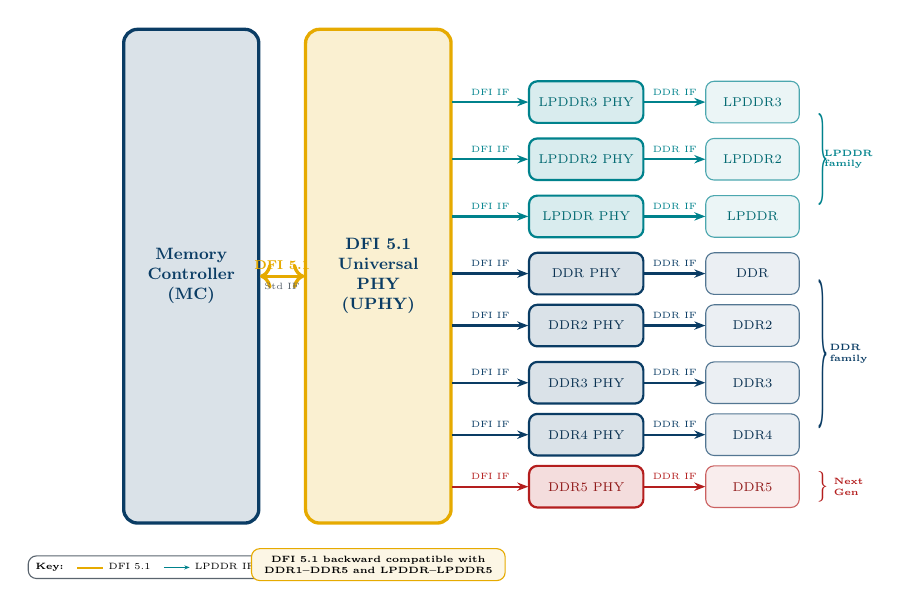
\begin{tikzpicture}[scale=0.66, transform shape,
   every node/.style={font=\scriptsize}]

  %% Memory Controller
  \node[rectangle,rounded corners=5pt,
        draw=ddrblue,fill=ddrblue!15,very thick,
        minimum width=26mm,minimum height=95mm,
        font=\small\bfseries,text=ddrblue,align=center]
    (mc) at (-3.6,0) {Memory\\Controller\\(MC)};

  %% UPHY
  \node[rectangle,rounded corners=5pt,
        draw=ddrgold,fill=ddrgold!18,very thick,
        minimum width=28mm,minimum height=95mm,
        font=\small\bfseries,text=ddrblue,align=center]
    (uphy) at (0,0) {DFI 5.1\\Universal\\PHY\\(UPHY)};

  %% DFI 5.1 bus
  \draw[ddrgold,very thick,<->]
    (mc.east) -- node[above,font=\scriptsize\bfseries,ddrgold]{DFI 5.1}
                  node[below,font=\tiny,ddrgray]{Std IF} (uphy.west);

  \def\phyX{4.0}
  \def\ddrX{7.2}

  \foreach \name/\y/\pcol/\dcol in {
    LPDDR3/ 3.35/ddrteal/ddrteal,
    LPDDR2/ 2.25/ddrteal/ddrteal,
    LPDDR/  1.15/ddrteal/ddrteal,
    DDR/    0.05/ddrblue/ddrblue,
    DDR2/  -0.95/ddrblue/ddrblue,
    DDR3/  -2.05/ddrblue/ddrblue,
    DDR4/  -3.05/ddrblue/ddrblue,
    DDR5/  -4.05/ddrred/ddrred}{

    \node[rectangle,rounded corners=3pt,
          draw=\pcol,fill=\pcol!15,thick,
          minimum width=22mm,minimum height=8mm,
          text=\pcol!80!black,align=center]
      (phy\name) at (\phyX,\y) {\name\ PHY};

    \node[rectangle,rounded corners=3pt,
          draw=\dcol!70,fill=\dcol!8,
          minimum width=18mm,minimum height=8mm,
          text=\dcol!80!black,align=center]
      (mem\name) at (\ddrX,\y) {\name};

    \draw[\pcol,thick,-{Stealth[length=4pt]}]
      (uphy.east |- phy\name.west) --
      node[above,font=\tiny,\pcol]{DFI IF} (phy\name.west);

    \draw[\dcol,thick,-{Stealth[length=4pt]}]
      (phy\name.east) -- node[above,font=\tiny,\dcol]{DDR IF} (mem\name.west);
  }

  %% Curly braces: mirror + top-to-bottom = bulge faces RIGHT, label on right
  %% Braces as text nodes — unaffected by transform shape
  \node[font=\large,ddrteal,rotate=0] at (8.55, 2.25)
    {\textcolor{ddrteal}{\scalebox{1}[4.2]{\}}}};
  \node[font=\tiny\bfseries,ddrteal,align=left] at (9.05, 2.25) {LPDDR\\family};

  \node[font=\large,ddrblue,rotate=0] at (8.55,-1.50)
    {\textcolor{ddrblue}{\scalebox{1}[6.8]{\}}}};
  \node[font=\tiny\bfseries,ddrblue,align=left] at (9.05,-1.50) {DDR\\family};

  \node[font=\large,ddrred,rotate=0] at (8.55,-4.05)
    {\textcolor{ddrred}{\scalebox{1}[1.4]{\}}}};
  \node[font=\tiny\bfseries,ddrred,align=left] at (9.05,-4.05) {Next\\Gen};

  %% Legend
  \node[draw=ddrgray,fill=white,rounded corners=3pt,
        inner sep=4pt,align=left,font=\tiny]
    at (-3.6,-5.6) {%
      \textbf{Key:}\quad
      \tikz\draw[ddrgold,very thick](0,0)--(0.5,0); DFI 5.1\quad
      \tikz\draw[ddrteal,thick,-{Stealth[length=3pt]}](0,0)--(0.5,0); LPDDR IF\quad
      \tikz\draw[ddrblue,thick,-{Stealth[length=3pt]}](0,0)--(0.5,0); DDR IF
    };

  %% Compat note
  \node[draw=ddrgold,fill=ddrgold!10,rounded corners=3pt,
        inner sep=4pt,align=center,font=\tiny\bfseries,text width=46mm]
    at (0,-5.55) {DFI 5.1 backward compatible with\\
                  DDR1--DDR5 and LPDDR--LPDDR5};

\end{tikzpicture}
\end{frame}

\end{document}